\section*{1}
\subsection*{a}
The Hamiltonian is
\eql{
\ham &= -\vec{\mu}\cdot\vec{B}\\
&= \gamma \br{B_x\spin_x + B_z\spin_z}\\
&= \gamma \br{B_x\sigma_x+B_z\sigma_z}\\
&= \gamma \begin{pmatrix}
    B_z & B_x\\
    B_x&-B_z
\end{pmatrix}
}
Where $\gamma = \frac{g\mu_B}{\h}$. The Eigen-values and normalized Eigen-vectors are
\eql{
\det\br{\ham - I_2\la}&=\det\begin{pmatrix}
    \gamma B_z-\la & \gamma B_x\\
    \gamma B_x& -\gamma B_z-\la
\end{pmatrix}\\
&= \br{\gamma B_z+\la}\br{-\gamma B_z-\la}-\gamma^2B_x^2\\
&= \la^2-\gamma^2\br{B_x^2+B_z^2}\\
&= \la^2-\gamma^2|\vec{B}|^2\\
&= \br{\la+\gamma|\vec{B}|}\br{\la-\gamma|\vec{B}|}\\
\implies \la &= \pm \gamma |\vec{B}|\\
}
If $\la = \gamma|\vec{B}|$ then the Eigen equation is
\eql{
\ham \cv{a b} &= \gamma|\vec{B}|\cv{a b}\\
\begin{pmatrix}
    B_z -|\vec{B}| & B_x\\
    B_x & -B_z -|\vec{B}|
\end{pmatrix} \cv{a b} &= \cv{0 0}
}
By inspection, the first row gives us (letting $a=B_x$) that
\eql{
\ket{\gamma |\vec{B}|} &= \begin{pmatrix}
B_x\\ |\vec{B}|-B_z
\end{pmatrix}
}
If $\la = -\gamma | \vec{B} |$ then the Eigen equation is
\eql{
\ham \cv{a b} &= -\gamm|\vec{B}|\cv{a b}\\
\begin{pmatrix}
    B_z +|\vec{B}| & B_x\\
    B_x & -B_z +|\vec{B}|
\end{pmatrix} \cv{a b} &= \cv{0 0}
}
Again, letting $a=B_x$, we get
\eq{
\ket{-\gamma |\vec{B}|} &= \begin{pmatrix}
B_x\\ -|\vec{B}|-B_z
\end{pmatrix}
}

\subsection*{b}
In the limit where $B_z \gg B_x$ the Eigen-values become
\eql{
\la &= \pm \gamma |\vec{B}|\\
&= \pm \gamma \sqrt{B_z^2+B_x^2}\\
&\approx \pm \gamma B_z
}
The Eigen-vectors become the following
\eql{
\ket{\gamma |\vec{B}|} &= \begin{pmatrix}
B_x\\ |\vec{B}|-B_z
\end{pmatrix}\\
&= B_x\begin{pmatrix}
1\\ \frac{|\vec{B}|-B_z}{B_x}
\end{pmatrix}\\
&\approx B_x\begin{pmatrix}
1\\ \frac{B_z-B_z}{B_x}
\end{pmatrix}\\
&\approx B_x\begin{pmatrix}
1\\ 0
\end{pmatrix}
}
We're free to rescale Eigen-vectors and write
\eql{
\ket{\gamma B_z} &\approx \cv{1 0}
}
Similarly
\eql{
\ket{-\gamma |\vec{B}|} &= \begin{pmatrix}
B_x\\ -|\vec{B}|-B_z
\end{pmatrix}\\
&= -(|\vec{B}|+B_z)\begin{pmatrix}
\frac{B_x}{|\vec{B}|+B_z} \\ 1
\end{pmatrix}\\
&\approx -2B_z\begin{pmatrix}
\frac{B_x}{2B_z}\\ 1
\end{pmatrix}\\
&\approx -2B_z\begin{pmatrix}
0\\ 1
\end{pmatrix}
}
Again, rescaling, we can write
\eql{
\ket{-\gamma B_z} &\approx \cv{0 1}
}
\subsection*{c}
In the limit where $B_x \gg B_z$ the Eigen-values become
\eql{
\la &= \pm \gamma |\vec{B}|\\
&= \pm \gamma \sqrt{B_z^2+B_x^2}\\
&\approx \pm \gamma B_x
}
The Eigen-vectors become the following
\eql{
\ket{\gamma |\vec{B}|} &= \begin{pmatrix}
B_x \\ |\vec{B}| - B_z
\end{pmatrix}\\
&= B_x \begin{pmatrix}
    1 \\ \frac{B_x}{|\vec{B}|-B_z}
\end{pmatrix}\\
&\approx B_x \begin{pmatrix}
    1 \\ \frac{B_x}{B_x-B_z}
\end{pmatrix}\\
&\approx B_x \begin{pmatrix}
    1 \\ 1
\end{pmatrix}
}
Rescaling
\eql{
\ket{\gamma B_x} &\approx \cv{1 1}
}
Similarly
\eql{
\ket{-\gamma |\vec{B}|} &= \begin{pmatrix}
    B_x \\ -|\vec{B}| - B_z
\end{pmatrix}\\
&= B_x \begin{pmatrix}
    1 \\ \frac{B_x}{-|\vec{B}|-B_z}
\end{pmatrix}\\
&\approx B_x \begin{pmatrix}
    1 \\ \frac{B_x}{-B_x-B_z}
\end{pmatrix}\\
&\approx B_x \begin{pmatrix}
    1 \\ -1
\end{pmatrix}
}
Rescaling the Eigen-vector
\eql{
\ket{-\gamma B_x} &\approx \cv{1 -1}
}
\subsection*{d}
\eql{
\ham &= A\sigma_z\\
\begin{pmatrix}
    B_z & B_x\\
    B_x & -B_z
\end{pmatrix}
&=\begin{pmatrix}
    a & b\\
    c & d
\end{pmatrix}\sz\\
&= \begin{pmatrix}
    a & -b\\
    c & -d
\end{pmatrix}
}
So we can write $A$ as
\eql{
A &= \begin{pmatrix}
    B_z & -B_x\\
    B_x & B_z
\end{pmatrix}
}
The characteristic equation becomes
\eql{
0 &= (B_z -\la)^2+B_x^2\\
iB_x &= \pm (B_z - \la)\\
\implies \la &= B_z \pm i B_x
}
The Eigen-equations are then
\eql{
\begin{pmatrix}
    -iB_x & -B_x\\
    B_x & -iB_x
\end{pmatrix}\cv{a b} &= \cv{0 0}\\
\begin{pmatrix}
    iB_x & -B_x\\
    B_x & iB_x
\end{pmatrix}\cv{a b} &= \cv{0 0}\\
}
We will pick $a$ to be $-1$ and $1$, respectively, so the Eigen-vectors are
\eql{
\ket{B_z+iB_x} &= \cv{-1 i}\\
\ket{B_z-iB_x} &= \cv{1 i}
}
The $z$ direction can be written in the Eigen-basis as follows
\eq{
1/2 \cv{1 i} - 1/2 \cv{-1 i} &= \cv{1 0}\\
1/2 (\ket{B_z-iB_x} - \ket{B_z+iB_x}) &= \ket{\gamma B_z}
}
\subsection*{e}
The expectation value of spin in the $z$ direction of the positive energy Eigen-state of the original Hamiltonian is
\eq{
<\hat{S}_z>_{\ket{\gamma |\vec{B}|}} &= <\gamma |\vec{B}||\hat{S}_z|\gamma |\vec{B}|>\\
&=\begin{pmatrix}
    B_x & |\vec{B}|-B_z
\end{pmatrix} \Sz \begin{pmatrix}
    B_x\\|B|-B_z
\end{pmatrix}\\
&= \frac{\h}{2}\begin{pmatrix}
    B_x & |\vec{B}|-B_z
\end{pmatrix}\begin{pmatrix}
    B_x \\ B_z - |\vec{B}|
\end{pmatrix}\\
&= \h B_z(|\vec{B}|-2B_z)
}
\pagebreak
\section*{2}
The plot is below
\begin{figure}[h]
    \centering
    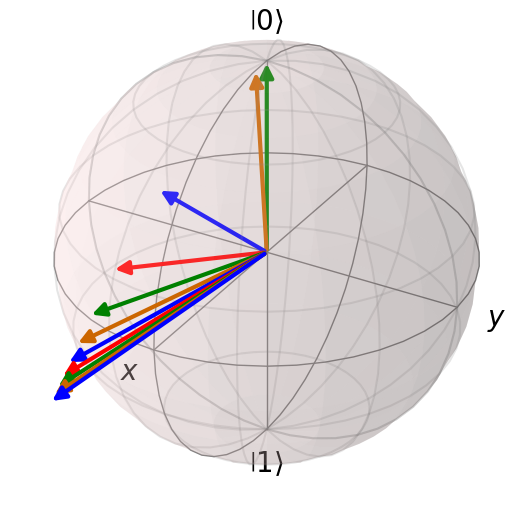
\includegraphics[width=0.75\linewidth]{Resources//245//Homework 2/245 Homework 2 Problem 2.png}
    \caption{Bloc Sphere for various $B_x/B_z$}
    \label{fig:enter-label}
\end{figure}
\section*{3}
\subsection*{a}
The Eigen-values and normalized Eigen-vectors of $\sigma_x$ are
\eql{
\sigma_x \cv{a b} &= \la \cv{a b}\\
\br{\sigma_x - \la I_2 }\cv{a b}&=0\\
\implies \det\br{\sx - \la I_2 }&=\br{\la+1}\br{\la-1} = 0\\
\implies \la &= \pm 1
}
When $\la = 1$
\eql{
\sigma_x \cv{a b} &= \cv{a b}\\
\sx \cv{a b} &= \cv{a b}\\
\cv{b a} &= \cv{a b}\\
\implies a &= b\\
\implies \cv{a b} &= \frac{1}{\sqrt{2}}\cv{1 1}
}
When $\la = -1$
\eql{
\sigma_x\cv{a b} &= -\cv{a b}\\
\sx \cv{a b} &= -\cv{a b}\\
\cv{b a} &= -\cv{a b}\\
\implies a &= -b\\
\implies \cv{a b} &= \frac{1}{\sqrt{2}}\cv{1 -1}
}
\subsection*{b}
The Eigen-values and normalized Eigen-vectors of $\sigma_y$ are
\eql{
\sigma_y \cv{a b} &= \la \cv{a b}\\
\br{\sigma_y - \la I_2 }\cv{a b}&=0\\
\implies \det\br{\sy - \la I_2 }&=\br{\la+1}\br{\la-1} = 0\\
\implies \lambda &= \pm 1
}
When $\la = 1$
\eql{
\sigma_y \cv{a b} &= \cv{a b}\\
\sy \cv{a b} &= \cv{a b}\\
i\cv{-b a} &= \cv{a b}\\
\implies ia &= b\\
\implies \cv{a b} &= \frac{1}{\sqrt{2}}\cv{1 i}
}
When $\la = -1$
\eql{
\sigma_y\cv{a b} &= -\cv{a b}\\
\sy \cv{a b} &= -\cv{a b}\\
i\cv{-b a} &= -\cv{a b}\\
\implies ia &= -b\\
\implies \cv{a b} &= \frac{1}{\sqrt{2}}\cv{1 -i}
}
\subsection*{c}
The Eigen-values and normalized Eigen-vectors of $\sigma_z$ are
\eql{
\sigma_z \cv{a b} &= \la \cv{a b}\\
\br{\sigma_z - \la I_2 }\cv{a b}&=0\\
\implies \det\br{\sz - \la I_2 }&=-\br{\la+1}\br{\la-1} = 0\\
\implies \lambda &= \pm 1
}
When $\la = 1$
\eql{
\sigma_z \cv{a b} &= \cv{a b}\\
\sz \cv{a b} &= \cv{a b}\\
\cv{a -b} &= \cv{a b}\\
\implies -b &= b\\
\implies \cv{a b} &= \cv{1 0}
}
When $\la = -1$
\eql{
\sigma_z\cv{a b} &= -\cv{a b}\\
\sz \cv{a b} &= -\cv{a b}\\
\cv{a -b} &= -\cv{a b}\\
\implies a &= -a\\
\implies \cv{a b} &= \cv{0 1}
}
\section*{4}
\subsection*{a,b and c}
\eql{
\sigma_x^2 &= \sx^2\\
&=\I\\
\sigma_y^2 &= \sy^2\\
&=\I\\
\sigma_z^2 &= \sz^2\\
&= \I\\
}
\subsection*{d}
\eql{
\exp\br{i\theta \sigma_x}&=\sum_n\frac{1}{n!}\br{i\theta\sigma_x}^n\\
&= \sum_n\frac{1}{n!}\br{i\theta\sx}^n\\
&= \sigma_x\sum_n\frac{1}{(2n+1)!}(i\theta)^{(2n+1)}+ I_2\sum_n\frac{1}{(2n)!}(i\theta)^{2n}\\
&= \sigma_x\sinh\br{i\theta} + I_2\cosh\br{i\theta}\\
&= \begin{pmatrix}
\cosh\br{i\theta} & \sinh\br{i\theta}\\
\sinh\br{i\theta} & \cosh\br{i\theta}
\end{pmatrix}
}
\subsection*{e}
\eql{
\exp\br{i\theta \sigma_y}&=\sum_n\frac{1}{n!}\br{i\theta\sigma_y}^n\\
&= \sum_n\frac{1}{n!}\br{i\theta\sy}^n\\
&= i\begin{pmatrix}
\cosh\br{i\theta} & -\sinh\br{i\theta}\\
\sinh\br{i\theta} & \cosh\br{i\theta}
\end{pmatrix}
}
\subsection*{f}
\eql{
\exp\br{i\theta \sigma_z}&=\sum_n\frac{1}{n!}\br{i\theta\sigma_z}^n\\
&= \sum_n\frac{1}{n!}\br{i\theta\sz}^n\\
&= \begin{pmatrix}
\cosh\br{i\theta}+\sinh\br{i\theta} & 0\\
0 & \cosh\br{i\theta}-\sinh\br{i\theta}
\end{pmatrix}
}
\section*{5}
\subsection*{a}
The Hamiltonian of a system with resonant drive is (assuming $\phi = 0$)
\eq{
\frac{\ham}{\h} &=\frac{\w_0}{2}\sigma_z + \Omega\cos(\w t)\sigma_x\\
}
The general solution to the Schrodinger equation is
\eq{
\ket{\psi(t)} &= a\ex{-i \frac{\w_0}{2}t}\ket{0} + b\ex{i \frac{\w_0}{2}t}\ket{1}\\
}
Plugging this into Schrodinger's equation we get
\eq{
i\partial_t \ket{\psi} &= (i\dot{a} + a \frac{\w_0}{2}t)\ket{0}+(i\dot{b}-b \frac{\w_0}{2}t)\ket{1}\\
\frac{\ham}{\h} \ket{\psi} &= (a\frac{\w_0}{2}+b\Omega \cos(\w t)\ex{i\frac{\w_0}{2}t})\ex{-i\frac{\w_0}{2}t}\ket{0}\\
&+(-b\frac{\w_0}{2}+a\Omega \cos(\w t)\ex{-i\frac{\w_0}{2}t})\ex{i\frac{\w_0}{2}t}\ket{1} 
}
We then apply the RWA to get the ODE
\eq{
 i\partial_t \ket{\phi} &= \frac{\Omega}{2} \begin{pmatrix}
     0 & \ex{-i\delta t}\\
     \ex{i \delta t} & 0
 \end{pmatrix}\ket{\phi}
}
Where $\ket{\phi}$ is the variable vector of $a$ and $b$. We'll rewrite this as
\eq{
i\dot{a} &= b\frac{\Omega}{2}\ex{-i\delta t}\\
i\dot{b} &= a\frac{\Omega}{2}\ex{i\delta t}
}
Differentiating the first equation and substituting into the second equation gives us
\eq{
\frac{2i}{\Omega}(\Ddot{a}+i\delta\dot{a})\ex{i\delta t} &= \dot{b}\\
\frac{-2}{\Omega}(\Ddot{a}+i\delta\dot{a})\ex{i\delta t} &= a\frac{\Omega}{2}\ex{i\delta t}\\
\Ddot{a}+i\delta\dot{a}+\frac{\Omega^2}{2^2}a &= 0
}
The characteristic polynomial is
\eq{
0&= r^2 + i\delta r + \frac{\Omega^2}{2^2}\\
\implies r &= \frac{i}{2}( \delta \pm \Omega')
}
So the general solution to the ODE is
\eq{
a(t) &= c_1\ex{ \frac{i}{2}(\Omega' + \delta)t} + c_2\ex{ \frac{i}{2}(\delta-\Omega')t}\\
\dot{a}(t) &= \frac{i}{2}c_1(\Omega'+\delta)\ex{\frac{i}{2}(\Omega'+\delta)t} + \frac{i}{2}c_2(\delta-\Omega')\ex{\frac{i}{2}(\delta-\Omega')t}\\
b(t) &= \frac{-1}{\Omega}c_1(\Omega'+\delta)\ex{\frac{i}{2}(\Omega'+3\delta)t} + \frac{-1}{\Omega}c_2(\delta-\Omega')\ex{\frac{i}{2}(\Omega'+\delta)t}\\
}
Plugging in the initial conditions
\eq{
b(0) &= \frac{-1}{\Omega}c_1(\Omega'+\delta)-\frac{1}{\Omega}c_2(\delta-\Omega')=0\\
a(0) &= c_1 + c_2 = 1\\
a(t)&=\frac{\Omega'-\delta}{2\Omega'-\delta}\ex{ \frac{i}{2}(\Omega' + \delta)t}+(1-\frac{\Omega'-\delta}{2\Omega'-\delta})\ex{ \frac{i}{2}(\delta-\Omega')t}\\
}
We can now calculate the modulus of $a(t)$
\eq{
a*(t)a(t) &= (\frac{\Omega'-\delta}{2\Omega'-\delta})^2 + (1-\frac{\Omega'-\delta}{2\Omega'-\delta})^2\\
&+2(\frac{\Omega'-\delta}{2\Omega'-\delta})(1-\frac{\Omega'-\delta}{2\Omega'-\delta})[\ex{i\Omega't}+\ex{-i\Omega't}]\\
&= (\frac{\Omega'-\delta}{2\Omega'-\delta})^2 + (1-\frac{\Omega'-\delta}{2\Omega'-\delta})^2\\
&+4(\frac{\Omega'-\delta}{2\Omega'-\delta})(1-\frac{\Omega'-\delta}{2\Omega'-\delta})(1-2\sin^2(\frac{\Omega'}{2}t))\\
&= 1-\frac{\Omega^2}{\Omega'^2}\sin^2(\frac{\Omega'}{2}t)
}
\subsection*{b}
If the probability of being in $\ket{0}$ is $1-\frac{\Omega^2}{\Omega'^2}\sin^2(\frac{\Omega'}{2}t)$, then the probability of being in $\ket{1}$ is $P_1 = 1- P_0 = \frac{\Omega^2}{\Omega'^2}\sin^2(\frac{\Omega'}{2}t)$. When $\Omega't = \pi$ the probability becomes $P_1 = \frac{\Omega^2}{\Omega'^2}=\frac{\Omega^2}{\Omega^2+\delta^2}$.
Normalizing the distribution we get that $\Omega = \frac{1}{\pi}$, the plot is below.
\begin{figure}[h]
    \centering
    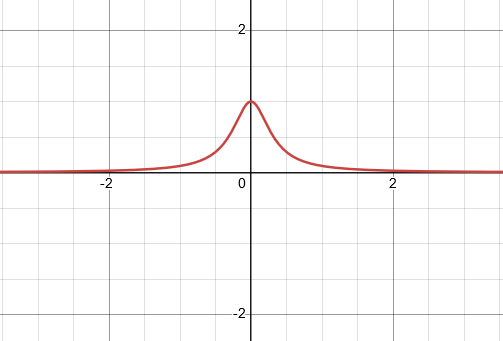
\includegraphics[width=0.5\linewidth]{Resources//245//Homework 2/245 Homework 2 Problem 5.png}
    \label{fig:enter-label}
\end{figure}